\documentclass[12pt,a4paper,onecolumn]{exam}

\usepackage{amsmath}
\usepackage{amsthm}
\usepackage{amssymb}
\usepackage{graphicx}
\usepackage{float}
\usepackage{geometry}
\usepackage{tikz}
\usepackage[skins]{tcolorbox}
\usepackage{listings}
\usepackage{xcolor}
\usepackage{hyperref}
\usepackage{multirow}
\usepackage{adjustbox}
\usepackage{booktabs}
\usepackage[font=small]{caption}
\usepackage{subcaption}

% --- Code Listing Colors ---
\definecolor{codegreen}{rgb}{0,0.6,0}
\definecolor{codegray}{rgb}{0.5,0.5,0.5}
\definecolor{codepurple}{rgb}{0.58,0,0.82}
\definecolor{backcolour}{rgb}{0.95,0.95,0.92}

% --- Code Listing Style ---
\lstdefinestyle{mystyle}{
    backgroundcolor=\color{backcolour},
    commentstyle=\color{codegreen},
    keywordstyle=\color{magenta},
    numberstyle=\tiny\color{codegray},
    stringstyle=\color{codepurple},
    basicstyle=\ttfamily\footnotesize,
    breaklines=true,
    captionpos=b,
    keepspaces=true,
    numbers=left,
    numbersep=2pt,
    showspaces=false,
    showstringspaces=false,
    showtabs=false,
    tabsize=1
}

\newcommand{\questionheader}[1]{%
  \begin{tcolorbox}[
    enhanced,
    colback=black,
    coltext=white,
    boxrule=0pt,
    fontupper=\Large\bfseries,
    arc=4mm
  ]
  #1
  \end{tcolorbox}%
}

\lstset{style=mystyle, language=Python}

\begin{document}

\begingroup
    \centering
    \LARGE E1 244 Detection and Estimation Theory\\
    \LARGE Assignment 5\\[0.5em]
    \large Dwaipayan Haldar\par
    \large \today\\[0.5em]
\endgroup
\noindent\rule{\textwidth}{0.5pt}
\printanswers
\renewcommand{\solutiontitle}{\noindent\textbf{Ans:}\enspace}

%----------------------------------------------------------------------
\questionheader{Problem 1}
%----------------------------------------------------------------------

\begin{solution}

Given:
\[
f(y \mid H_0) = \begin{cases} c|y-1| & \text{if } |y| \leq 1, \\ 0 & \text{otherwise,} \end{cases}
\qquad
f(y \mid H_1) = \begin{cases} \dfrac{|y-2|}{8} & \text{if } |y| \leq 2, \\ 0 & \text{otherwise.} \end{cases}
\]

\textbf{(a) Finding the constant $c$:}

By the definition of a pdf, $\int f(y \mid H_0)\,dy = 1$:
\[
\int_{-1}^{1} c|y-1|\,dy = 1.
\]
Since $y \in [-1,1]$ implies $y-1 \leq 0$, we have $|y-1| = 1-y$. Thus:
\[
c\int_{-1}^{1}(1-y)\,dy = c\left[y - \frac{y^2}{2}\right]_{-1}^{1}
= c\left[\left(1-\tfrac{1}{2}\right) - \left(-1-\tfrac{1}{2}\right)\right] = 2c = 1.
\]
\[
\boxed{c = \frac{1}{2}.}
\]

\textbf{(b) Bayes Decision Rule:}

With costs $C_{00},\,C_{10},\,C_{01},\,C_{11}$ and priors $\Pr(H_0),\,\Pr(H_1)$, the Bayes (LRT) rule is:
\[
\frac{f(y \mid H_1)}{f(y \mid H_0)} \underset{H_0}{\overset{H_1}{\gtrless}} \gamma,
\qquad \gamma = \frac{(C_{10}-C_{00})\,\Pr(H_0)}{(C_{01}-C_{11})\,\Pr(H_1)}.
\]

With $c = 1/2$, note $|y-2| = 2-y$ for $y \leq 2$ and $|y-1|=1-y$ for $y \leq 1$.

\begin{itemize}
\item For $y \in [-2,-1) \cup (1,2]$: only $f(y\mid H_1)>0$, so $\hat{H}=H_1$ by default.
\item For $y \in [-1,1]$ (common support region):
\[
\frac{f(y\mid H_1)}{f(y\mid H_0)}
= \frac{\tfrac{2-y}{8}}{\tfrac{1}{2}(1-y)}
= \frac{2-y}{4(1-y)}
\underset{H_0}{\overset{H_1}{\gtrless}} \gamma.
\]
Cross-multiplying:
\[
(2-y) \underset{H_0}{\overset{H_1}{\gtrless}} 4(1-y)\gamma
\implies y(4\gamma-1) \underset{H_0}{\overset{H_1}{\gtrless}} 4\gamma-2
\implies y \underset{H_0}{\overset{H_1}{\gtrless}} \frac{4\gamma-2}{4\gamma-1}.
\]
\end{itemize}

The complete Bayes decision rule is:
\[
\hat{H} = \begin{cases}
H_1 & \text{if } |y| \leq 1 \text{ and } y \geq \dfrac{4\gamma-2}{4\gamma-1}, \\[6pt]
H_1 & \text{if } 1 < |y| \leq 2, \\[4pt]
H_0 & \text{otherwise.}
\end{cases}
\]

\textbf{(c) MAP and ML Criteria:}

\underline{MAP rule} (set $\gamma = \Pr(H_0)/\Pr(H_1)$): In the common region $|y|\leq 1$,
\[
f(y\mid H_1)\,\Pr(H_1) \underset{H_0}{\overset{H_1}{\gtrless}} f(y\mid H_0)\,\Pr(H_0)
\implies
(2-y)\,\Pr(H_1) \underset{H_0}{\overset{H_1}{\gtrless}} 4(1-y)\,\Pr(H_0).
\]

\underline{ML rule} (set $\gamma = 1$): Then $\dfrac{4\gamma-2}{4\gamma-1} = \dfrac{2}{3}$. In the common region,
\[
(2-y) \underset{H_0}{\overset{H_1}{\gtrless}} 4(1-y)
\implies 3y \underset{H_0}{\overset{H_1}{\gtrless}} 2
\implies y \underset{H_0}{\overset{H_1}{\gtrless}} \frac{2}{3}, \quad -1 \leq y \leq 1.
\]
Outside the common region, $\hat{H}=H_1$ for $1 < |y| \leq 2$.

\end{solution}

%----------------------------------------------------------------------
\questionheader{Problem 2}
%----------------------------------------------------------------------

\begin{solution}

Given $X_1,X_2 \overset{\text{i.i.d.}}{\sim} f(x) = e^{-x}\mathbf{1}_{\{x\geq 0\}}$, with $H_0: Y=X_1$ vs $H_1: Y=X_1+X_2$.

\textbf{(a) Distribution of $Y$ under $H_1$:}

Under $H_1$, $Y = X_1 + X_2$. Computing the CDF via conditioning:
\begin{align*}
F_Y(y) &= P(Y \leq y) = P(X_1 + X_2 \leq y) \\
&= \int_{0}^{y} P(X_2 \leq y - x_1 \mid X_1)\,e^{-x_1}\,dx_1 \\
&= \int_{0}^{y} \bigl[1 - e^{-(y-x_1)}\bigr]e^{-x_1}\,dx_1 \\
&= \int_{0}^{y} e^{-x_1}\,dx_1 - \int_{0}^{y} e^{-y}\,dx_1 \\
&= \bigl(1-e^{-y}\bigr) - y\,e^{-y}.
\end{align*}
Differentiating:
\[
f(y \mid H_1) = \frac{d}{dy}\bigl(1 - e^{-y} - ye^{-y}\bigr)
= e^{-y} - \bigl(-ye^{-y} + e^{-y}\bigr) = ye^{-y}, \quad y \geq 0.
\]
This is a Gamma(2,1) (Erlang-2) distribution.

\textbf{(b) N-P Test with $P_F = \alpha$:}

Under $H_0$, $Y \sim \text{Exp}(1)$, so $f(y\mid H_0) = e^{-y}\mathbf{1}_{\{y\geq 0\}}$. The likelihood ratio is:
\[
\frac{f(y\mid H_1)}{f(y\mid H_0)} = \frac{ye^{-y}}{e^{-y}} = y \underset{H_0}{\overset{H_1}{\gtrless}} \gamma, \quad y \geq 0.
\]
\textit{Threshold}: Setting $P_F = \alpha$:
\[
P_F = \int_{\gamma}^{\infty} e^{-y}\,dy = e^{-\gamma} = \alpha \implies \gamma = -\ln\alpha.
\]
The N-P test is $y \underset{H_0}{\overset{H_1}{\gtrless}} -\ln P_F$ for $y \geq 0$.

\textit{Detection Probability} (with $\gamma = -\ln\alpha$):
\begin{align*}
P_D &= \int_{\gamma}^{\infty} ye^{-y}\,dy
= \bigl[-ye^{-y}\bigr]_{\gamma}^{\infty} + \int_{\gamma}^{\infty} e^{-y}\,dy
= \gamma e^{-\gamma} + e^{-\gamma} = (\gamma+1)\,e^{-\gamma}.
\end{align*}
Since $e^{-\gamma} = P_F$:
\[
\boxed{P_D = P_F\,(1 - \ln P_F).}
\]

\textbf{(c) ROC Curve:}

The ROC is given by $P_D = P_F(1-\ln P_F)$ for $P_F \in [0,1]$.

\begin{figure}[H]
    \centering
    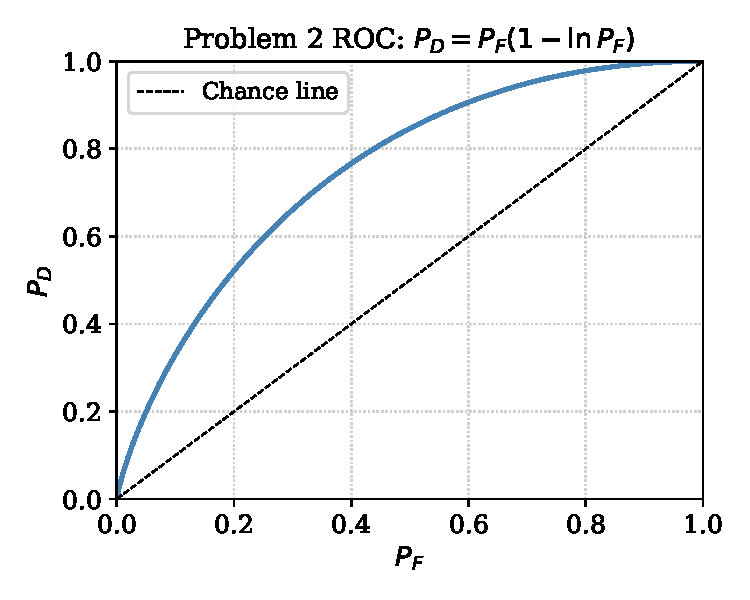
\includegraphics[width=0.55\textwidth]{roc_p2.pdf}
    \caption{ROC curve for Problem~2: $P_D = P_F(1-\ln P_F)$.}
    \label{fig:roc_p2}
\end{figure}

\end{solution}

%----------------------------------------------------------------------
\questionheader{Problem 3}
%----------------------------------------------------------------------

\begin{solution}

The payoff table is:
\begin{center}
\begin{tabular}{ccc}
\toprule
Plant Early & Frost Occurs & Profit \\
\midrule
Yes & No  & $+5{,}00{,}000$ \\
Yes & Yes & $-2{,}00{,}000$ \\
No  & Yes & $0$ \\
No  & No  & $0$ \\
\bottomrule
\end{tabular}
\end{center}

Define $H_0$: Frost occurs ($\Pr(H_0)=0.6$) and $H_1$: Frost does not occur ($\Pr(H_1)=0.4$).

\textbf{(a) Bayes Decision (Maximum Expected Profit):}

Expected profit if Plant Early (PE):
\begin{align*}
\mathbb{E}[\text{Profit} \mid \text{PE}]
&= 5{,}00{,}000 \times \Pr(H_1) - 2{,}00{,}000 \times \Pr(H_0) \\[4pt]
&= 5{,}00{,}000 \times 0.4 - 2{,}00{,}000 \times 0.6 \\[4pt]
&= 2{,}00{,}000 - 1{,}20{,}000 \;=\; 80{,}000.
\end{align*}
Expected profit if No PE:
\[
\mathbb{E}[\text{Profit} \mid \text{No PE}] = 0.
\]
Since $80{,}000 > 0$, the Bayes decision is: \textbf{Plant Early.}

\textbf{(b) Minmax Decision:}

\begin{itemize}
\item Plant Early: worst-case profit $= -2{,}00{,}000$ (when frost occurs).
\item Do Not Plant Early: worst-case profit $= 0$.
\end{itemize}
Minmax maximises the worst-case outcome: $0 > -2{,}00{,}000$.\\
Minmax decision: \textbf{Do Not Plant Early.}

\textbf{(c) Personal Choice of Criterion:}

I would personally choose the \textbf{Bayes criterion}. It leverages the known prior probability of frost ($0.6$) to maximise expected profit over many trials. The minmax criterion is overly conservative: it guards against the worst case regardless of how likely that case actually is.

\end{solution}

%----------------------------------------------------------------------
\questionheader{Problem 4}
%----------------------------------------------------------------------

\begin{solution}

Given:
\[
f(y \mid H_0) = \begin{cases} \dfrac{y+3}{18} & \text{if } |y| \leq 3, \\ 0 & \text{otherwise,} \end{cases}
\qquad
f(y \mid H_1) = \begin{cases} \dfrac{1}{4} & \text{if } y \in [0,4], \\ 0 & \text{otherwise.} \end{cases}
\]
The supports overlap on $[0,3]$.

\textbf{(a)(i) Bayes Rule --- Uniform Costs, Equal Priors:}

With $C_{01}=C_{10}=1$, $C_{00}=C_{11}=0$, and $\Pr(H_0)=\Pr(H_1)=\tfrac{1}{2}$, the threshold $\gamma=1$ and the Bayes rule reduces to the ML rule $f(y\mid H_1) \underset{H_0}{\overset{H_1}{\gtrless}} f(y\mid H_0)$.

In the common region $[0,3]$:
\[
\frac{1}{4} \underset{H_0}{\overset{H_1}{\gtrless}} \frac{y+3}{18}
\implies 4.5 \underset{H_0}{\overset{H_1}{\gtrless}} y+3
\implies y \underset{H_1}{\overset{H_0}{\gtrless}} 1.5.
\]

\begin{tcolorbox}[colback=gray!10, boxrule=0.4pt]
\textbf{Final Decision Rule:}
\[
\delta(y) = \begin{cases}
H_0 & \text{if } -3 \leq y < 0, \\
H_1 & \text{if } 0 \leq y \leq 1.5, \\
H_0 & \text{if } 1.5 < y \leq 3, \\
H_1 & \text{if } 3 < y \leq 4.
\end{cases}
\]
\end{tcolorbox}

\textbf{(a)(ii) Minimum Bayes Risk:}

\begin{align*}
J &= \frac{1}{2}\,P(\hat{H}=H_1 \mid H_0) + \frac{1}{2}\,P(\hat{H}=H_0 \mid H_1) \\
&= \frac{1}{2}\int_{0}^{1.5}\frac{y+3}{18}\,dy + \frac{1}{2}\int_{1.5}^{3}\frac{1}{4}\,dy.
\end{align*}
Computing:
\[
\int_{0}^{1.5}\frac{y+3}{18}\,dy
= \left[\frac{y^2}{36}+\frac{y}{6}\right]_{0}^{1.5}
= \frac{2.25}{36}+\frac{9}{36} = \frac{11.25}{36},
\qquad
\int_{1.5}^{3}\frac{1}{4}\,dy = \frac{1.5}{4} = \frac{13.5}{36}.
\]
\[
\boxed{J = \frac{1}{2}\cdot\frac{11.25}{36} + \frac{1}{2}\cdot\frac{13.5}{36}
= \frac{24.75}{72} \approx 0.3437.}
\]

\textbf{(b)(i) Min-Max Rule --- Uniform Costs:}

For a threshold $\eta \in [0,3]$ (decide $H_1$ for $y \leq \eta$ in $[0,3]$, and always $H_1$ for $y\in(3,4]$):
\[
J(\eta,0) = \int_{0}^{\eta}\frac{y+3}{18}\,dy = \frac{\eta^2}{36}+\frac{\eta}{6},
\qquad
J(\eta,1) = \int_{\eta}^{3}\frac{1}{4}\,dy = \frac{3-\eta}{4}.
\]
The min-max threshold equates both risk components:
\[
\frac{\eta^2}{36}+\frac{\eta}{6} = \frac{3-\eta}{4}
\implies \eta^2 + 6\eta + 9\eta - 27 = 0
\implies \eta^2 + 15\eta - 27 = 0.
\]
\[
\eta = \frac{-15+\sqrt{225+108}}{2} = \frac{-15+\sqrt{333}}{2} \approx \frac{-15+18.25}{2} \approx 1.624.
\]

\begin{tcolorbox}[colback=gray!10, boxrule=0.4pt]
\textbf{Final Min-Max Decision Rule:}
\[
\delta(y) = \begin{cases}
H_0 & \text{if } -3 \leq y < 0, \\
H_1 & \text{if } 0 \leq y \leq 1.624, \\
H_0 & \text{if } 1.624 < y \leq 3, \\
H_1 & \text{if } 3 < y \leq 4.
\end{cases}
\]
\end{tcolorbox}

\textbf{(b)(ii) Min-Max Risk:}
\[
\boxed{J_{\text{minmax}} = \frac{3-\eta}{4} = \frac{3-1.624}{4} \approx 0.344.}
\]

\textbf{(c) ROC Curve:}

Parameterising by threshold $\eta \in [0,3]$ (decide $H_1$ for $y\in[0,\eta]\cup(3,4]$):
\[
P_F = \int_{0}^{\eta}\frac{y+3}{18}\,dy = \frac{\eta^2}{36}+\frac{\eta}{6},
\qquad
P_D = \int_{0}^{\eta}\frac{1}{4}\,dy + \int_{3}^{4}\frac{1}{4}\,dy = \frac{\eta}{4}+\frac{1}{4}.
\]
Eliminating $\eta$ from $P_F$: $\eta^2 + 6\eta - 36P_F = 0 \Rightarrow \eta = -3 + 3\sqrt{1+4P_F}$. Substituting:
\[
\boxed{P_D = \frac{-2 + 3\sqrt{1+4P_F}}{4}.}
\]
The ROC starts at $(P_F,P_D)=(0,\,0.25)$ when $\eta=0$ and ends at $(0.75,\,1)$ when $\eta=3$.

\begin{figure}[H]
    \centering
    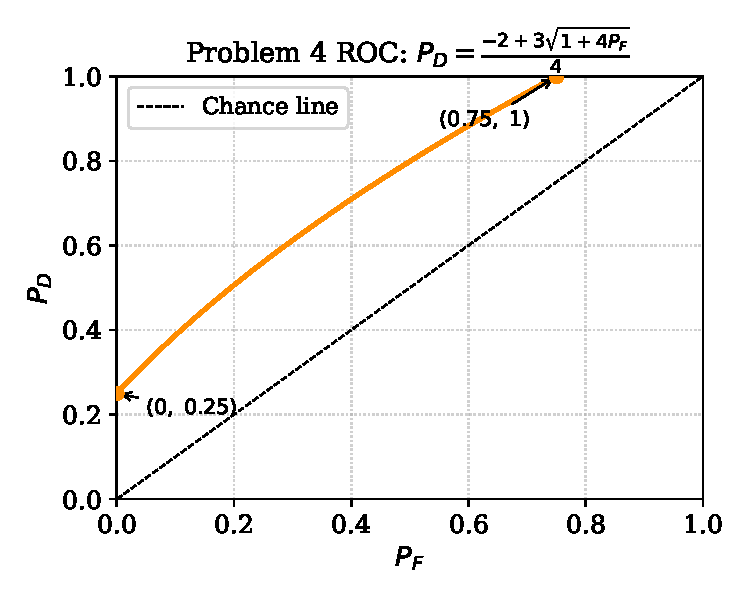
\includegraphics[width=0.55\textwidth]{roc_p4.pdf}
    \caption{ROC curve for Problem~4: $P_D = \frac{-2+3\sqrt{1+4P_F}}{4}$.}
    \label{fig:roc_p4}
\end{figure}

\end{solution}

%----------------------------------------------------------------------
\questionheader{Problem 5}
%----------------------------------------------------------------------

\begin{solution}

$Y = U + \lambda\theta$, where $U \sim \mathrm{Uniform}[-1,1]$, $0\leq\lambda\leq2$.
Under $H_0$ ($\theta=0$): $f(y\mid H_0)=\tfrac{1}{2}\,\mathbf{1}_{\{|y|\leq1\}}$.
Under $H_1$ ($\theta=1$): $f(y\mid H_1)=\tfrac{1}{2}\,\mathbf{1}_{\{\lambda-1\leq y\leq\lambda+1\}}$.

The likelihood ratio is:
\[
L(y) = \frac{f(y\mid H_1)}{f(y\mid H_0)}
= \begin{cases}
0      & \text{if } -1 \leq y < \lambda-1, \\
1      & \text{if } \lambda-1 \leq y \leq 1, \\
\infty & \text{if } 1 < y \leq \lambda+1.
\end{cases}
\]

\textbf{(a) N-P Decision Rule and ROC:}

Since $L(y) \in \{0,1,\infty\}$ only, varying $\eta$ yields only two non-trivial cases:

\textbf{Case 1} ($\eta \leq 1$): Decide $H_1$ when $L(y)\geq\eta$, i.e.\ $y\in[\lambda-1,\lambda+1]$:
\[
P_F = \int_{\lambda-1}^{1}\tfrac{1}{2}\,dy = 1 - \frac{\lambda}{2}, \qquad P_D = 1.
\]

\textbf{Case 2} ($\eta > 1$): Decide $H_1$ only when $L(y)=\infty$, i.e.\ $y\in(1,\lambda+1]$:
\[
P_F = 0, \qquad P_D = \int_{1}^{\lambda+1}\tfrac{1}{2}\,dy = \frac{\lambda}{2}.
\]

The N-P ROC consists of only two discrete points:
\[
\left(0,\;\frac{\lambda}{2}\right) \quad \text{and} \quad \left(1-\frac{\lambda}{2},\;1\right).
\]
\textit{Reason}: $L(y)$ is piecewise constant (values $0,1,\infty$), so there is no intermediate threshold that shifts $P_F$ continuously. Any threshold $\eta\in(0,1)$ gives the same $(P_F,P_D)$ as $\eta=1$, and any $\eta\in(1,\infty)$ gives the same as $\eta\to\infty$.

\textbf{(b) Alternate Deterministic Rule:}

At $\eta=1$ the overlapping region $[\lambda-1,1]$ can be partially assigned. Define:
\[
\delta(y) = \begin{cases}
H_1 & \text{if } y \in (1,\lambda+1] \;\cup\; [\lambda-1,\,\lambda-1+t], \\
H_0 & \text{otherwise,}
\end{cases}
\quad 0 \leq t \leq 2-\lambda.
\]
Then:
\[
P_F = \int_{\lambda-1}^{\lambda-1+t}\frac{1}{2}\,dt = \frac{t}{2},
\qquad
P_D = \frac{t}{2} + \int_{1}^{\lambda+1}\frac{1}{2}\,dt = \frac{t}{2} + \frac{\lambda}{2}.
\]
\[
\boxed{P_D = P_F + \frac{\lambda}{2}.}
\]
This is a line segment connecting $\bigl(0,\,\tfrac{\lambda}{2}\bigr)$ to $\bigl(1-\tfrac{\lambda}{2},\,1\bigr)$, i.e.\ the two N-P points.

Endpoints for each $\lambda$:
\begin{itemize}
\item $\lambda=0.5$: from $(0,\;0.25)$ to $(0.75,\;1)$.
\item $\lambda=1$:   from $(0,\;0.5)$  to $(0.5,\;1)$.
\item $\lambda=1.5$: from $(0,\;0.75)$ to $(0.25,\;1)$.
\item $\lambda=2$:   single point $(0,\;1)$ (perfect detector).
\end{itemize}

\begin{figure}[H]
    \centering
    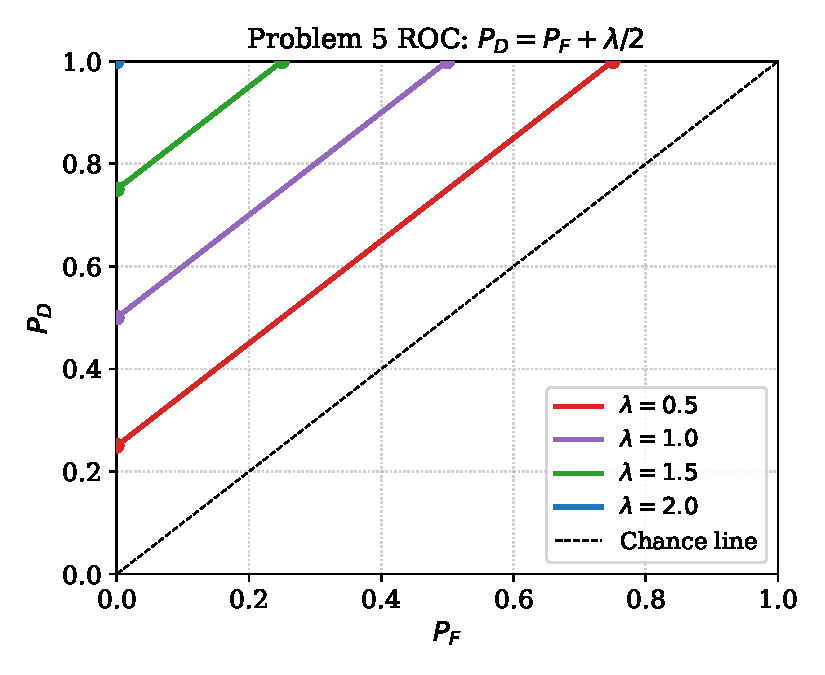
\includegraphics[width=0.6\textwidth]{roc_p5.pdf}
    \caption{ROC curves for Problem~5 with $\lambda=0.5,\,1,\,1.5,\,2$.}
    \label{fig:roc_p5}
\end{figure}

\end{solution}

%----------------------------------------------------------------------
\questionheader{Problem 6}
%----------------------------------------------------------------------

\begin{solution}

A Poisson counting process $N(t)$ is observed over $[0,T]$. The pmf of $n=N(T)$ given rate $\lambda$ is:
\[
p(n \mid \lambda) = \frac{(\lambda T)^{n}\,e^{-\lambda T}}{n!}.
\]

\textbf{(a) Sufficient Statistic:}

By the Neyman--Fisher factorisation theorem, $T(Y)$ is sufficient for $\lambda$ if
$p(n\mid\lambda) = g(T(Y),\lambda)\cdot h(Y)$.
Write:
\[
p(n\mid\lambda) = \underbrace{\frac{(\lambda T)^{n}}{n!}}_{g(n,\,\lambda)} \cdot \underbrace{e^{-\lambda T}}_{h(\lambda)}.
\]
Here $g$ depends on $\lambda$ only through $T(Y)=n=N(T)$, and $h$ does not depend on $Y$ at all.
Hence $N(T)$ is a sufficient statistic for $\lambda$. $\blacksquare$

\textbf{(b) LRT --- Uniform Costs, Arbitrary Priors:}

The likelihood ratio is:
\[
L(Y) = \frac{p(N(T)\mid\lambda_1)}{p(N(T)\mid\lambda_0)}
= \left(\frac{\lambda_1}{\lambda_0}\right)^{N(T)} e^{-(\lambda_1-\lambda_0)T}.
\]
For uniform costs ($C_{01}=C_{10}$), the Bayesian LRT is $L(Y)\underset{H_0}{\overset{H_1}{\gtrless}} P_0/P_1$.
Taking logarithms:
\[
N(T)\ln\frac{\lambda_1}{\lambda_0} \underset{H_0}{\overset{H_1}{\gtrless}} \ln\frac{P_0}{P_1} + (\lambda_1-\lambda_0)T \;\triangleq\; \tilde{\eta}.
\]
\textbf{If $\lambda_1>\lambda_0$} (divide by $\ln(\lambda_1/\lambda_0)>0$):
\[
N(T) \underset{H_0}{\overset{H_1}{\gtrless}}
\frac{\ln(P_0/P_1)+(\lambda_1-\lambda_0)T}{\ln(\lambda_1/\lambda_0)} \triangleq \eta.
\]
\textbf{If $\lambda_0>\lambda_1$} (inequality reverses):
\[
N(T) \underset{H_1}{\overset{H_0}{\gtrless}} \eta.
\]

\textbf{(c) Total Probability of Error:}

\[
P(E) = P_1\,P(H_0\text{ decided}\mid H_1) + P_0\,P(H_1\text{ decided}\mid H_0).
\]

\textbf{Case $\lambda_1>\lambda_0$} (decide $H_1$ if $N(T)\geq\eta$):
\[
P(E) = P_1\sum_{n=0}^{\eta-1}\frac{e^{-\lambda_1 T}(\lambda_1 T)^{n}}{n!}
      + P_0\sum_{n=\eta}^{\infty}\frac{e^{-\lambda_0 T}(\lambda_0 T)^{n}}{n!}.
\]

\textbf{Case $\lambda_0>\lambda_1$} (decide $H_1$ if $N(T)\leq\eta$):
\[
P(E) = P_1\sum_{n=\eta}^{\infty}\frac{e^{-\lambda_1 T}(\lambda_1 T)^{n}}{n!}
      + P_0\sum_{n=0}^{\eta-1}\frac{e^{-\lambda_0 T}(\lambda_0 T)^{n}}{n!}.
\]

\end{solution}

\end{document}
